\documentclass[a4paper]{jpconf}

\usepackage{graphicx}
\usepackage{bm}        % for math
\usepackage{amssymb}   % for math
\usepackage{amsfonts}
\usepackage{amsmath}
\usepackage{epsfig}
\usepackage{units}
\usepackage{cite}
%\usepackage[numbers,square,sort&compress]{natbib}
\usepackage[utf8]{inputenc}
\usepackage[T1]{fontenc}
\usepackage{color}
\usepackage{hyperref}
\usepackage{lineno}
\linenumbers

%particles
\newcommand{\jpsi}{\rm J/$\psi$}
\newcommand{\psip}{$\psi^\prime$}
\newcommand{\jpsiDY}{\rm J/$\psi$\,/\,DY}
\newcommand{\chic}{$\chi_{\rm c}$}
\newcommand{\pip}{$\pi^{+}$}
\newcommand{\pim}{$\pi^{-}$}
\newcommand{\pizero}{$\pi^{0}$}
\newcommand{\kap}{K$^{+}$}
\newcommand{\kam}{K$^{-}$}
\newcommand{\pbar}{$\rm\overline{p}$}
\newcommand{\ccbar}{\ensuremath{\mathrm{c\overline{c}}}}
\newcommand{\bbbar}{\ensuremath{\mathrm{b\overline{b}}}}
\newcommand{\Dzero}{\ensuremath{\mathrm{D^{0}}}}
\newcommand{\Dzerobar}{\ensuremath{\mathrm{\overline{D}^{0}}}}
\newcommand{\Dpm}{\ensuremath{\mathrm{D^{\pm}}}}
\newcommand{\Ds}{\ensuremath{\mathrm{D_{s}^{\pm}}}}
\newcommand{\Dstar}{\ensuremath{\mathrm{D^{*\pm}}}}

%collision systems
\newcommand{\pp}{pp}
\newcommand{\pPb}{p--Pb}
\newcommand{\PbPb}{Pb--Pb}

%detectors
\newcommand{\ezdc}{$E_{\rm ZDC}$}

%units
\newcommand{\GeVc}{GeV/$c$}
\newcommand{\GeVcsq}{GeV/$c^2$}

%others
\newcommand{\degree}{$^{\rm o}$}
\newcommand{\s}{\ensuremath{\sqrt{s}}}
\newcommand{\snn}{\ensuremath{\sqrt{s_{\rm NN}}}}
\newcommand{\y}{\ensuremath{y}}
\newcommand{\pt}{\ensuremath{p_{\rm T}}}
\newcommand{\dedx}{d$E$/d$x$}
\newcommand{\dndy}{d$N$/d$y$}
\newcommand{\dndydpt}{${\rm d}^2N/({\rm d}y {\rm d}p_{\rm t})$}
\newcommand{\zpar}{\ensuremath{z_{||}}}
\newcommand{\zpargen}{\ensuremath{z_{||}^{\mathrm{part}}}}
\newcommand{\zpardet}{\ensuremath{z_{||}^{\mathrm{det}}}}
\newcommand{\ptchjet}{\ensuremath{p_{\mathrm{T,ch\, jet}}}}
\newcommand{\ptjet}{\ensuremath{p_{\mathrm{T,jet}}}}
\newcommand{\ptchjetgen}{\ensuremath{p_{\mathrm{T,ch\,jet}}^{\mathrm{part}}}}
\newcommand{\ptchjetdet}{\ensuremath{p_{\mathrm{T,ch\,jet}}^{\mathrm{det}}}}
\newcommand{\ptd}{\ensuremath{p_{\mathrm{T,D}}}}
\newcommand{\ptdgen}{\ensuremath{p_{\mathrm{T,D}}^{\mathrm{part}}}}
\newcommand{\ptddet}{\ensuremath{p_{\mathrm{T,D}}^{\mathrm{det}}}}
\newcommand{\antikt}{anti-\ensuremath{k_{\mathrm{T}}}}
\newcommand{\Antikt}{Anti-\ensuremath{k_{\mathrm{T}}}}
\newcommand{\kt}{\ensuremath{k_{\mathrm{T}}}}
\newcommand{\pthard}{\ensuremath{p_{\mathrm{T,hard}}}}

\begin{document}
\title{Measurement of D-meson tagged jets in pp collisions at 7 TeV with ALICE}

\author{Salvatore Aiola, for the ALICE Collaboration}

\address{Physics Department, Yale University, 266 Whitney Avenue, New Haven, CT 06511}

\ead{salvatore.aiola@cern.ch}

\begin{abstract}
We present the current status of the measurement of jets that contain a D meson (D-tagged jets) with \mbox{ALICE}.
D-meson candidates, identified via their hadronic decay channels, are combined with the other charged tracks reconstructed by the central tracking system, 
using the anti-$k_{\rm T}$ jet-finding algorithm.
We extract the yield of D-tagged jets through an invariant mass analysis of the D-meson candidates.
A Monte Carlo simulation has been used to extract the detector performance and validate the signal extraction techniques.
\end{abstract}

\section{Introduction}
At hadron colliders, charm quarks are produced as a result of a hard scattering of partons. Like lighter quarks or gluons, charm quarks
fragment into collimated sprays of hadrons called \emph{jets}. The charm content of the jet is conserved throughout the fragmentation process,
which is dominated by Quantum Chromo-Dynamics (QCD).
In the final state, the charm content can be identified by looking for the presence of charmed hadrons.

The measurement of the charm jet production cross section in \pp\ collisions is an important, sensitive test of perturbative QCD (pQCD) calculations.
In particular, at the LHC energies, the measurement of charm production at low \pT\ probes the parton distribution functions (PDFs)
of the proton at small values of parton fractional momentum, $x$, and squared momentum transfer, $Q^2$, 
a kinematical region where pQCD calculations suffer from large uncertainties.

Heavy quarks are also an ideal probe of the hot and dense matter, 
known as the Quark-Gluon Plasma (QGP)~\cite{STAR:2005a, PHENIX:2005a}, 
that is created in ultra-relativistic heavy-ion collisions. 
Hard scattered partons, including heavy quarks, interact with the QGP, which increases their virtuality and interferes with the
parton shower (\emph{jet quenching})~\cite{PHENIX:2008b, CMS:2012b, ALICE:2015a}.
At low energy, comparable to the charm mass, the charm quark is expected
to interact less strongly with the QGP, a phenomenon known as the dead-cone effect~\cite{Dokshitzer:2001}.

Most of the charm measurements performed at the LHC so far report the production cross section of hadrons
containing heavy quarks~\cite{ALICE:2012d, LHCb:2013a, ATLAS:2016a, ALICE:2016b}.
Measuring the kinematic observables of jets implies integrating out some of the hadronization degrees of freedom. 
Since hadronization is a highly non-perturbative process, known only with large uncertainties~\cite{dEnterria:2014}, 
reducing its influence in the measurement may improve comparisons with pQCD calculations.
Furthermore, the details of the charm quark fragmentation can be the subject of a more careful study in which the kinematic observables 
of both the jet and the charmed hadron are available at the same time. In particular the measurement of the fraction of the jet momentum carried 
by the charmed hadron can provide important insights on the charm production mechanism~\cite{CDF:1990, UA1:1990, STAR:2009a, ATLAS:2012d}.

\section{The ALICE Experiment}
ALICE is the experiment dedicated to the study of heavy-ion collisions at the LHC.
The central barrel detectors ($\lvert \eta\rvert \lesssim 1$) are positioned within a large solenoid magnet, with a
field $B = 0.5$~T, parallel to the beam line.
PID and low-momentum tracking capabilities are among the strongest points of ALICE.
The \emph{Inner Tracking System} (ITS) is a six-layer silicon detector that allows the precise determination of the primary vertex 
and the displacement of secondary vertices of weak decays.
%with a resolution better than $75\, \rm \mu m$ for transverse momenta $\pT > 1$~\GeVc.
The main tracking detector is the \emph{Time Projection Chamber} (TPC), which, combined with the ITS, allows reconstruction of tracks 
from low momentum ($\pT\approx0.15$~\GeVc) to high momentum
($\pT\approx100$~\GeVc) with good momentum resolution and tracking efficiency.
%a momentum resolution ranging from about 1\% to 3\% (low and intermediate momentum) and tracking
%efficiency better than 80\% for $\pT>0.5$~\GeVc.
Several detectors contribute to the Particle Identification (PID) capabilities of ALICE. 
In particular in this analysis we use the \dedx\ measurement from the TPC and
the \emph{Time Of Flight} (TOF) detector. The TOF detector is a large area array of Multigap Resistive Plate Chambers (MRPC).
%, covering the full azimuth and the pseudorapidity range $\lvert \eta\rvert \lesssim 0.9$.
The TPC \dedx\ measurement provides good hadron identification at low momentum ($\pT\lesssim0.7$~\GeVc) and 
in the relativistic rise region ($\pT\gtrsim2$~\GeVc);
TOF provides PID in the intermediate momentum range,
up to about $3$~\GeVc\ depending on the mass of the particle.
%up to $2.5$~\GeVc\ for pions and kaons, and up to $4$~\GeVc\ for protons.
A full description of ALICE and of its performance during LHC Run-1 is available at Ref.~\cite{ALICE:2014b}.

\section{Analysis procedures}
The analysis relies on the well established D meson reconstruction techniques~\cite{ALICE:2012d, ALICE:2016a}, as well as
jet reconstruction methods~\cite{ALICE:2013c, ALICE:2015a, ALICE:2015e}, both developed by the ALICE Collaboration during Run-1.
%The analysis procedures are outlined in the following subsections.

\subsection{Monte Carlo simulations}
%ALICE plans to measure D-tagged jets in \pp\ collisions at $\s=$~7, 8 and 13 TeV and in \pPb\ and \PbPb\ collisions at $\snn=$~5 TeV.
Two Monte Carlo simulations have been used to extract the detector performance and validate the analysis techniques.
PYTHIA6 (6.4.25)\cite{Sjostrand:2006} (tune Perugia-2011) has been used as event generator in both simulations.
For the first simulation (minimum-bias production) PYTHIA was configured to provide Minimum Bias (MB) \pp\ events at $\s=7$~TeV.
The simulated statistics (about 300 M events) is close to the total statistics accumulated by ALICE in MB \pp\ collisions
in 2010. In the second simulation (charm-enhanced production) PYTHIA was configured to retain only events with a \ccbar\ pair; the production
was split in eigth \pthard\ bins (\pT\ of the hard scatted parton). In addition, all D meson were forced
to decay hadronically. These settings allowed to gain enough statistical precision in the determination of the detector response with reasonable
computational costs.
In both cases, the PYTHIA events were then passed through the GEANT3~\cite{GEANT3-url} transport code with a detailed description of the ALICE apparatus,
as it was operated during the 2010 data-taking campaign.

\subsection{\Dzero-jet reconstruction}
%For more details about the tracking algorithm used by ALICE see Ref.~\cite{ALICE:2014b}.
Track quality cuts are applied to ensure good momentum resolution. 
\emph{Global} tracks have the best momentum and spatial resolution. They include at least three space point in the ITS (one of which in one of the two layers closest to the beam pipe).
%\emph{Silicon Pixel Detector} (SPD), which comprises the first two
%layers of the ITS, closer to the beam pipe, and at least a total of three in the whole ITS. 
They are required also to match with a track in the TPC, which has to include at least 70 space points.
% and no less than 80\% of the geometrically findable space points in the TPC. 
Decay products of the D mesons are found among this category of tracks.
Due to the non-uniform ITS response, the global-track efficiency reconstruction shows a strong azimuthal dependence.
To avoid interferences with the jet finding, some of the requirement on the ITS are lifted in the low-efficiency regions.
To improve momentum resolution, tracks without hits in the first few layers of the ITS, are \emph{constrained} to the primary vertex. 
This second collection of tracks is called \emph{hybrid}.

In this analysis \Dzero\ mesons ($m=1.865$~\GeVcsq, $c\tau=123\,\mu$m) are used to tag jets with charm content.
They are identified via their hadronic decay: \Dzero $\rightarrow$ \pip \kam (BR = 3.88\%)~\cite{PDG:2014}. Both the \Dzero\ and its
anti-particle $\overline{\Dzero}$~are considered.
%The first step of the analysis is to select events that contain at least one \Dzero-meson candidate.
\Dzero\ meson candidates are identified looking for unlike-sign (US) track pairs (\emph{daughters}) among all reconstructed \emph{global} tracks.
%In order to suppress the background from combinatorial matches, topological and PID cuts are applied.
The topological cuts select pairs that form a secondary vertex displaced from the reconstructed
primary vertex. PID on the \Dzero\ candidate daughters is used to reject pairs are not $\pi$K.
%The pairs that pass the selections are then used in the next steps.
The four-momentum of the \Dzero\ candidate is calculated summing the four-momenta of the two daughters.
When available, PID is used to assign mass values to the \Dzero\ candidate daughters. When PID is not conclusive,
the pair is used twice with either mass combinations (\pip \kam or \pim \kap). 

The four-momentum of each \Dzero\ candidate and all reconstructed \emph{hybrid} tracks
(excluding the two daughters of the \Dzero) are used as input of the \antikt\ jet-finding algorithm~\cite{Cacciari:2008c}.
%in its FASTJET~\cite{Cacciari:2012} implementation. 
Only jets containing the \Dzero\ candidates are selected.
For this study only the tracks of charged particles are used for jet reconstruction (\emph{charged| jets}). Since they miss the momentum
fraction carried by neutral particles, the kinematics of charged jets is less tightly correlated with the kinematics
of the original parton and depends more strongly on jet fragmentation. However, charged jets have better momentum resolution
and are less sensitive to pile-up; furthermore recent theoretical developments allow direct comparison with models~\cite{Thaler:2013}.

\subsection{Invariant mass analysis}
\Dzero\ candidates and their associated jets are then sorted according to jet momentum, \Dzero\ momentum and jet momentum
fraction carried by the \Dzero.
%, \zpar$=\frac{\bm{p}_{\rm jet}\cdot{\bm{p}}_{\rm D^0}}{\bm{p}_{\rm jet}^2}$.
Three different invariant mass analysis techniques have been developed and their performance compared.
\begin{description}
\item[Invariant mass fit] The \Dzero-jet candidates are divided in bins of \ptchjet\ and the invariant mass distribution of the \Dzero\ candidates is plot for each \ptchjet\ bin;
each candidate is given a weight corresponding to the inverse of its reconstruction efficiency $\epsilon(\ptd)$, extracted from a MC simulation (see Section~\ref{sect:detperf}).
The invariant mass distribution is fit using the sum of an exponential function (background) and a Gaussian (signal). The yield $N^{\rm \Dzero\hbox{-}jet}(\ptchjet)$ is extracted from
the fit parameters.
\item[Side-Band subtraction] The \Dzero-jet candidates are divided in bins of \ptd; for each bin the yield $N^{\rm \Dzero\hbox{-}jet}(\ptchjet,\ptd)$ is extracted by subtracting the
\ptchjet\ distribution in the side bands ($4\sigma_{\rm fit} < \lvert m - m_{\rm fit} \rvert < 8\sigma_{\rm fit}$) 
from the \ptchjet\ distribution in the peak area ($\lvert m - m_{\rm fit} \rvert < 2\sigma_{\rm fit}$); the peak position, peak width and background normalization are extracted 
by fitting the invariant mass distribution with an exponential + Gaussian function; the \ptd\ bins are summed over, weighted by the inverse of the reconstruction efficiency:
\begin{equation*}
N^{\rm \Dzero\hbox{-}jet}(\ptchjet)=\sum_{\ptd} \frac{1}{\epsilon(\ptd)} 
\left[N_{\rm peak}^{\rm \Dzero\hbox{-}jet}(\ptchjet,\ptd) - 
\frac{B_{\rm peak}^{\rm fit}}{B_{\rm SB}} 
N_{\rm SB}^{\rm \Dzero\hbox{-}jet}(\ptchjet,\ptd)\right],
\end{equation*}
where $B_{\rm peak}^{\rm fit}$ and $B_{\rm SB}$ are respectively the total background
in the peak area estimated by fitting the invariant mass distribution and the total
background in the side bands.
\item[Like-Sign subtraction] This method is analogous to the Side-Band method. In this case the background \ptchjet\ distribution is provided by the Like-Sign (LS) $\pi$K pairs and
subtracted from the corresponding Unlike-Sign (US) pairs:
\begin{equation*}
N^{\rm \Dzero\hbox{-}jet}(\ptchjet)=\sum_{\ptd} \frac{1}{\epsilon(\ptd)} 
\left[N_{\rm US, peak}^{\rm \Dzero\hbox{-}jet}(\ptchjet,\ptd) - 
\frac{B_{\rm US, SB}}{B_{\rm LS, SB}} 
N_{\rm LS, peak}^{\rm \Dzero\hbox{-}jet}(\ptchjet,\ptd)\right],
\end{equation*}
where $B_{\rm US, SB}$ and $B_{\rm LS, SB}$ are respectively the integral of
the side bands in the US and in the LS invariant mass distributions.
\end{description}

\section{Results}

\subsection{Detector performance}
\label{sect:detperf}
\begin{figure}[tb]
\centering
\begin{minipage}{.48\textwidth}
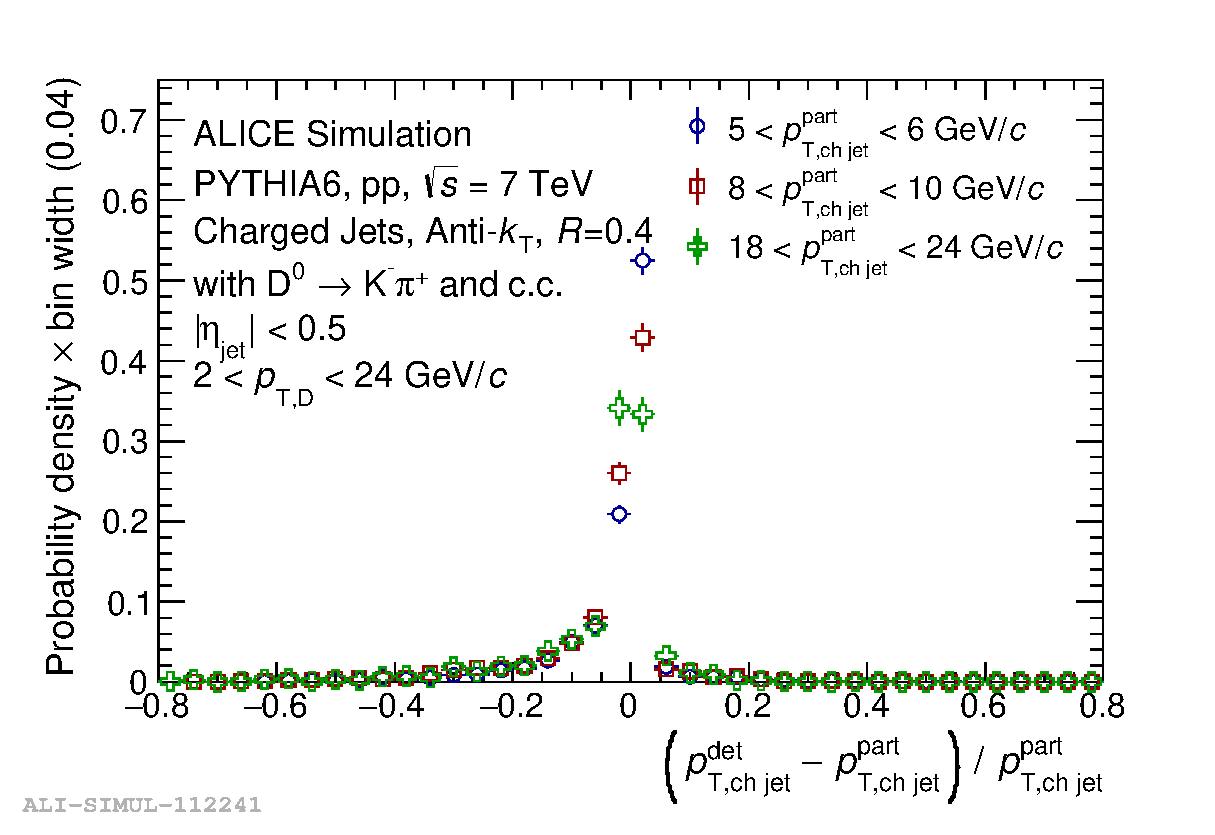
\includegraphics[width=\textwidth]{img/HQ16_Simulation_DetectorResponse}
\caption{\label{fig:HQ16_Simulation_DetectorResponse} Probability density distribution of the jet momentum shift between particle and detector level, for different ranges of \ptchjet.}
\end{minipage}\hspace{1pc}%
\begin{minipage}{.48\textwidth}
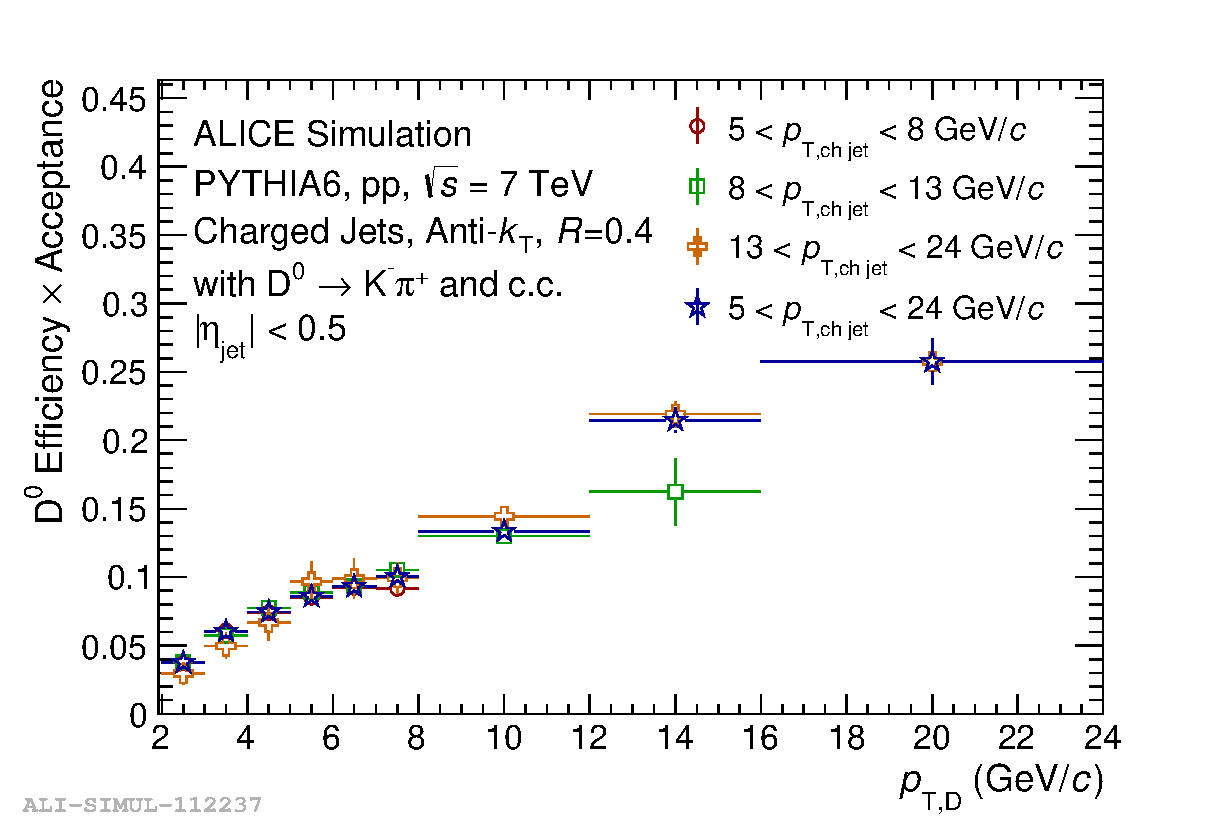
\includegraphics[width=\textwidth]{img/HQ16_Simulation_EfficiencyVsDPt}
\caption{\label{fig:HQ16_Simulation_EfficiencyVsDPt}Reconstruction efficiency of \Dzero\ mesons as a function of \ptd\ for different ranges of \ptchjet.}
\end{minipage} 
\end{figure}

The detector performance has been assessed using the charm-enhanced production. The D-tagged jets are identified at detector-level, 
%(i.e. after the GEANT3 detector response simulation)
%in an way equivalent to real data processing, except for the invariant mass analysis step. The real D mesons are selected among the candidates 
using the MC-truth information,
%The D-tagged jets are also identified 
and at generator-level.
%(i.e. PYTHIA events). 
Even-by-event, detector-level D-tagged jets are matched with their corresponding counterparts at generator-level.
This matched pairs are used to build a response matrix that relates detector-level observables with their corresponding generator-level observables. 
%This matrix can be used to correct detector-response distortions of the final distributions on an ensemble basis (\emph{unfolding}).
The jet momentum resolution and Jet Energy Scale (JES) shift have been quantified using the variable: 
\begin{equation}
\left( \ptchjetdet - \ptchjetgen \right) / \ptchjetgen,
\label{eq:energyshift}
\end{equation}
where \ptchjetdet\ and \ptchjetgen are the transverse momenta of the D-tagged jet at detector-level and at generator-level, respectively.
Its probability density distribution is shown in Fig.~\ref{fig:HQ16_Simulation_DetectorResponse} for three different ranges of \ptchjetgen. No significant dependence on \ptchjetgen\ is observed.
The shape of the distribution features a sharp peak at zero and is skewed towards negative values, due to tracking inefficiency (higher probability of
reconstructing jet momenta smaller than generated). The relative jet momentum resolution is quantified with the standard deviation
of the variable in Eq.~\ref{eq:energyshift}: $\sigma\approx11$~\%, slightly smaller compared to inclusive jets measured using the same data~\cite{ALICE:2015e}.
The mean~$\approx-3$~\% and median~$\approx0$ of the same distribution quantify the average JES shift.

The reconstruction efficiency is calculated as the ratio of the yield of reconstructed D-tagged jets over all generated D-tagged jets, as a function of generator-level observables.
The reconstruction efficiency is shown in Fig.~\ref{fig:HQ16_Simulation_EfficiencyVsDPt} as a function of \ptd\ for different ranges of \ptchjet. The reconstruction efficiency shows a stark dependence on \ptd, mainly due to
varying topological cuts. No significant dependence on \ptchjet\ is observed in the range $5<\ptchjet<24$~\GeVc.

\subsection{Invariant mass analysis}
\begin{figure}[tb]
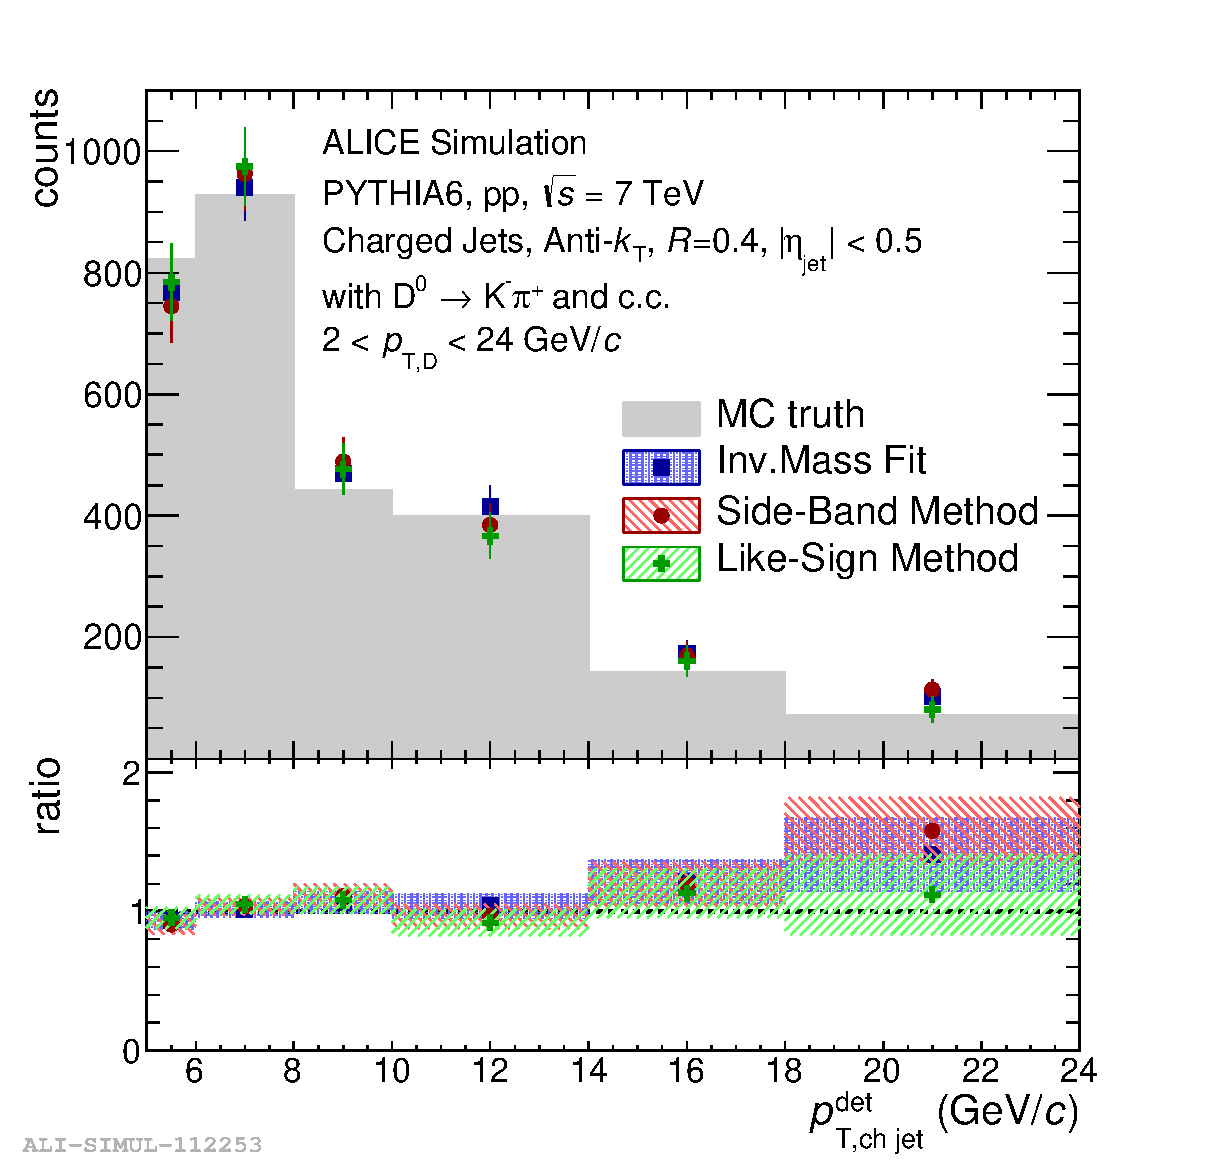
\includegraphics[width=.50\textwidth]{img/HQ16_Simulation_MethodComparison}\hspace{1pc}%
\begin{minipage}[b]{.50\textwidth}\caption{\label{fig:HQ16_Simulation_MethodComparison}\Dzero-jet signal yield extracted using the invariant mass fit (blue squares), side-band method (red circles) and like-sign method (green triangles)
compared with the MC truth (gray filled area). The bottom panel shows the ratio to the MC truth. The yields are corrected for the reconstruction efficiency but not for the distortions due to detector jet momentum resolution.}
\end{minipage}
\end{figure}

The minimum-bias production was used to validate the invariant mass analysis. 
%The D-tagged jets are identified at detector-level in an way equivalent to real data processing, including the invariant mass analysis step.
Figure~\ref{fig:HQ16_Simulation_MethodComparison} shows the D-tagged jet yields as a function of \ptchjetdet\ obtained using the invariant mass fit, 
side-band and like-sign methods, compared to the MC truth. All methods perform well and do not show any significant bias, beyond the statistical uncertainties assigned to each signal extraction method.

\section{Conclusions}
ALICE has a great potential for measuring jets with charm content tagged using fully reconstructed D mesons in pp collisions at $\s=7$~TeV, especially at low momentum ($\ptchjet \lesssim 30$~\GeVc),
as well as the intermediate momentum ($\ptjet\approx100$~\GeVc) and
low \ptd\ by exploiting the data collected at $\s=8,\,13$~TeV with the calorimeter triggers.
In \PbPb\ and \pPb\ collisions ALICE will study cold and hot nuclear matter effects
looking at the yields and fragmentation functions of low- and intermediate-momentum \Dzero-tagged jets.

The ALICE detector performance for \Dzero-tagged jets has been assessed using MC simulations
for pp collisions at $\s=7$~TeV. The \Dzero-jet momentum resolution has been measured to be about 11\%; the reconstruction efficiency is independent of \ptchjet\ and ranges from 5\% to 25\% as a function of \ptd.
Three methods have been implemented to extract the signal out of the $\pi$K combinatorial background: invariant mass fit, side-band and like-sign subtraction.
The three methods have been validated using a MC simulation and do not show biases larger than the statistical uncertainties.

\section*{References}
\bibliography{biblio}{}
\bibliographystyle{iopart-num}

\end{document}


